\documentclass[12pt]{article}
\usepackage{sbc-template}
\usepackage[utf8]{inputenc}
\usepackage{listings}
\usepackage{xcolor}
\usepackage[english]{babel}
\usepackage{graphicx}
\usepackage{url}

\lstdefinelanguage{JavaScript}{
  keywords={break, case, catch, continue, debugger, default, delete, do, else, finally, for, function, if, in, instanceof, new, return, switch, this, throw, try, typeof, var, void, while, with, let, const},
  morecomment=[l]{//},
  morecomment=[s]{/*}{*/},
  morestring=[b]',
  morestring=[b]",
  ndkeywords={class, export, boolean, throw, implements, import, this, extends, super},
  sensitive=true
}

\lstset{
  language=JavaScript,
  basicstyle=\ttfamily\small,
  keywordstyle=\color{blue},
  ndkeywordstyle=\color{orange},
  commentstyle=\color{gray},
  stringstyle=\color{green},
  breaklines=true,
  frame=single,
  captionpos=b,
  numbers=left,
  numberstyle=\tiny\color{gray},
  stepnumber=1,
  numbersep=5pt,
  showstringspaces=false,
  tabsize=2,
  backgroundcolor=\color{white},
  showspaces=false,
  showtabs=false,
  caption={Exemplo de código JavaScript},
  label={lst:exemplo-js}
}


\title{Using Generative AI on-premise in code review process}
\author{Pedro A. D. Kfuri\inst{1}, Advisor: Humberto Torres Marques Neto\inst{1} }
\address{
Instituto de Ciências Exatas e Informática \\
Pontifícia Universidade Católica de Minas Gerais (PUC MG)
  \email{pedrokfuri@outlook.com, humberto@pucminas.br}
}

\begin{document} 
\maketitle

\begin{resumo}
Este estudo explora a integração de IA Generativa para automatizar revisões de código em \textit{merge requests} do GitLab e do GitHub, utilizando o Ollama, um mecanismo de inferência de IA executado localmente. Um \textit{webhook} se conecta à API do GitLab ou do GitHub, analisando automaticamente as alterações no código, fornecendo feedback estruturado e ajudando na decisão de aprovação ou rejeição das solicitações. Essa solução melhora a eficiência das revisões, reduz o tempo de espera e mantém a privacidade dos dados ao operar em uma infraestrutura local. A abordagem proposta contribui para a engenharia de software assistida por IA ao simplificar a garantia de qualidade do código em ambientes de desenvolvimento colaborativo.
\end{resumo}

\begin{abstract}
This study explores the integration of Generative AI to automate code reviews in GitLab and Github merge requests using Ollama, an on-premise AI inference engine. A webhook connects to GitLab's or Github's API, automatically analyzing code changes, providing structured feedback, and helping to decide on request approval or rejection. This solution improves review efficiency, reduces waiting times, and maintains data privacy by operating on local infrastructure. The proposed approach contributes to AI-assisted software engineering by streamlining code quality assurance in collaborative development environments.
\end{abstract}

\section{Introduction}
In modern software engineering, code reviews are essential for maintaining code quality and ensuring team collaboration. However, as development teams expand and repositories grow, the manual code review process becomes increasingly time-consuming and prone to delays. These delays often stem from human availability constraints, leading to bottlenecks that hinder continuous integration and deployment. \cite{codereviewStudy}

The traditional approach to code reviews relies heavily on human reviewers, which poses scalability issues. As the volume of code increases, the capacity of human reviewers does not scale proportionally, resulting in inefficiencies. This mismatch can lead to prolonged development cycles and reduced productivity. \cite{integratingAIDevops}

Recent advancements in Generative AI present an opportunity to automate aspects of the code review process. By integrating AI-driven tools into existing workflows, it's possible to analyze code changes, provide feedback, and even approve or reject merge requests based on predefined criteria. This automation can enhance consistency and reduce the lead time for code integration.
\cite{aiDrivenAgile}

This proposal outlines the integration of Generative AI into GitLab\footnote{https://gitlab.com} and GitHub\footnote{https://github.com} workflows using Ollama\cite{ollama}, a locally deployed AI inference engine. By implementing a webhook that interfaces with GitLab's and GitHub's APIs, the system can analyze merge requests in real-time. This on-premise solution ensures data privacy while providing immediate, automated code reviews.

The integration aims to achieve several key outcomes: enhanced review consistency, reduced lead time for code integration, and adherence to best coding practices. By operating on-premise, the solution also addresses data privacy concerns associated with external AI services. These improvements are expected to streamline the development process and increase overall team productivity.

This research contributes to the field of AI-assisted software engineering by demonstrating the practical application of Generative AI in real-world development environments. The findings will provide insights into the efficiency and accuracy of automated code reviews, potentially influencing future practices in software development and AI integration.

\section{Background}

Artificial Intelligence (AI) and Machine Learning (ML) have significantly transformed DevOps, particularly in automating processes within Continuous Integration/Continuous Deployment (CI/CD) pipelines. AI-driven automation enhances efficiency, reduces manual effort, and improves software quality. Among the most promising advancements is the use of Large Language Models (LLMs) for automated code review, which provides real-time feedback, ensures coding standard adherence, and identifies potential security vulnerabilities. Faster feedback loops further streamline development cycles, contributing to higher productivity. \cite{AIDrivenDevops}

AI-enhanced DevOps, often referred to as "Intelligent DevOps," integrates predictive analytics, anomaly detection, and self-healing mechanisms into software development workflows. Studies highlight that organizations leveraging AI in DevOps experience substantial reductions in time-to-market and operational costs. AI-driven monitoring and diagnostics improve system reliability, allowing developers to focus on strategic tasks rather than repetitive debugging and error detection. \cite{interdisciplinaryAIMLDevopsAutomation}
    
\subsection{Code Review}
Code review, the practice of systematically evaluating peers' code to enhance quality, works as a mechanism for quality assurance and a platform for collaborative learning. By scrutinizing code changes, reviewers disseminate domain-specific knowledge, coding standards, and architectural insights, thereby reducing siloed expertise and enhancing long-term maintainability. This knowledge transfer is vital in both open-source and industrial contexts, where onboarding new contributors and maintaining coherent codebases are ongoing challenges. For instance, in large tech organizations, code review is integral to sustaining code health across millions of lines of code. \cite{codereviewStudy}

The automation of code review tasks has emerged as a key research frontier, addressing scalability and efficiency concerns. Techniques such as reviewer recommendation, automated comment generation, and predictive models for change approval aim to streamline processes while preserving review efficacy. Deep learning models, pre-trained on vast corpora of code and natural language, now simulate human-like feedback, though challenges like dataset noise and metric reliability persist. \cite{codereviewStudy}

While LLMs enhance technical efficiency in code reviews, their inability to engage in the reciprocal social dynamics of accountability such as mutual justification, reputation building, and collective norm reinforcement, risks eroding the socio-technical fabric of software development. A critical insight is the potential for adaptive hybrid workflows: LLMs could serve as first-line technical validators, automating routine checks, while reserving nuanced, context-sensitive decisions  to human reviewers. \cite{accountability}

\subsection{CICD/DevOps Integration}
Continuous Integration and Continuous Delivery (CI/CD) constitute a foundational framework within modern software development practices, designed to streamline the integration, testing, and deployment of code changes. In this paradigm, developers frequently merge their contributions into a shared repository, triggering automated workflows that compile the codebase, execute test suites, and validate functionality. Successful iterations progress to deployment phases, ensuring rapid, reliable delivery of software updates while minimizing disruptions. \cite{AIDrivenDevops}

Code review represents a critical phase in the CI/CD pipeline, serving as a gatekeeping mechanism prior to code integration. Traditionally, this stage relies on human reviewers to assess code for errors, adherence to coding standards, and potential security vulnerabilities. \cite{aiDrivenAgile}

\subsection{Gitlab/Github API}
GitLab and GitHub provide REST APIs to programmatically access diff contents, which are structured representations of code changes between commits, branches, or merge/pull requests. The APIs return JSON formatted data detailing modified files, including metadata and line-level additions/deletions.


\lstset{basicstyle=\ttfamily, frame=single, language=JavaScript}
\begin{lstlisting}[caption={Github Patches API Endpoint}, label={lst:github-patches}]
GET /pulls/{pull_number}/files
\end{lstlisting}

\lstset{basicstyle=\ttfamily, frame=single, language=JavaScript}
\begin{lstlisting}[caption={Gitlab Diffs API Endpoint}, label={lst:gitlab-diffs}]
GET /{id}/merge_requests/{iid}/changes
\end{lstlisting}

GitHub's Pull Request API outputs a files array with patch strings encoding line changes, while GitLab's Merge Request API organizes diffs into a changes array with diff fields. Key distinctions include GitHub's granular file statuses (e.g., added, modified) and GitLab's emphasis on commit-level change aggregation. Both enable automated analysis of code modifications but differ in data structuring and endpoint granularity, reflecting platform-specific workflows.

\subsection{Generative AI}
Generative AI has emerged as a transformative tool in CI/CD processes, particularly for automating code generation, test case synthesis, and deployment script optimization. AI-driven tools like DeepCode and Codacy employ machine learning to analyze codebases and suggest improvements. While not explicitly labeled as "generative", these tools align with generative AI principles by predicting and generating code fixes, enforcing standards, and identifying vulnerabilities through pattern recognition. Generative models could further enhance such workflows by autonomously drafting code snippets, generating test scenarios, or refining deployment strategies based on historical data. \cite{AIDrivenDevops}

\section{Related Work}
Recent advancements in Large Language Models (LLMs), such as GPT-4 and BERT, have introduced novel opportunities to enhance DevOps workflows through intelligent automation and natural language processing. One key application is automated code analysis and generation, where LLMs streamline code reviews and suggest optimizations. For instance, GitHub Copilot assists developers by generating context-aware code snippets, reducing manual effort and accelerating development cycles. Similarly, tools like DeepCode and Codacy leverage LLMs to detect vulnerabilities, enforce coding standards, and propose fixes by analyzing historical codebases. These models improve code quality while integrating seamlessly into CI/CD pipelines, enabling real-time feedback during continuous integration. \cite{aiStreamlinedCICD}

DACE \cite{automaticCR} is a deep learning model designed to automate code review by focusing on the differences between original and revised code segments. Unlike traditional methods that assess overall code similarity, DACE emphasizes the specific changes within code revisions, capturing the nuanced modifications developers make. By analyzing six open-source projects, the study demonstrated that DACE outperforms existing approaches in identifying meaningful code changes, thereby enhancing the efficiency and effectiveness of the code review process. This work underscores the potential of machine learning techniques in refining code review practices by targeting the granular aspects of code evolution.

In a broader exploration of AI's role in code review, \cite{evolvingLandscapeOfCodeReview} examined how tools like GitHub Copilot and Google's internal frameworks are reshaping software development workflows. The paper highlighted AI's capabilities in automating tasks such as bug detection, code refactoring, and enforcing coding standards, leading to improved software quality and developer productivity. However, it also cautioned against over-reliance on AI, pointing out risks like algorithmic bias and the potential for overlooking contextual nuances. Batte's analysis provides a comprehensive overview of the benefits and challenges associated with integrating AI into code review processes, emphasizing the need for balanced adoption strategies that combine technological advancements with human oversight.

Opportunities to research lie in the area of federated learning for training LLMs on decentralized DevOps datasets to preserve privacy, alongside developing multimodal LLMs capable of unified interpretation of code, logs, and user queries. Further exploration includes autonomous systems that dynamically optimize deployment pipelines through predictive resource allocation and adaptive rollback strategies. \cite{aiStreamlinedCICD}

\section{Methodology}
This implementation combines artificial intelligence with DevOps practices to build a server-side application that integrates with GitHub and GitLab. The application exposes an endpoint that is triggered whenever a pull or merge request is created, receiving a payload that contains the code changes. It then sends these changes to the Ollama API using a custom prompt and receives an AI-generated code review in response. Finally, the application posts the review as a comment on the corresponding pull or merge request page via the GitHub or GitLab API.

To enable this integration, webhooks must be manually configured in GitHub or GitLab. This involves specifying the server-side application's endpoint and selecting the appropriate access scope. The endpoint used is \textbf{https://tcc.pedrokfuri.com/webhook}. Refer to the Figures ~\ref{fig:gitlabwh} and ~\ref{fig:githubwh} for screenshots of the webhook configuration pages in GitLab and GitHub.

\begin{figure}[htbp]
    \centering
    
\includegraphics[width=1\textwidth]{gitlab-webhook.png}
    \caption{Gitlab Webhook}
    \label{fig:gitlabwh}
\end{figure}

\begin{figure}[htbp]
    \centering
    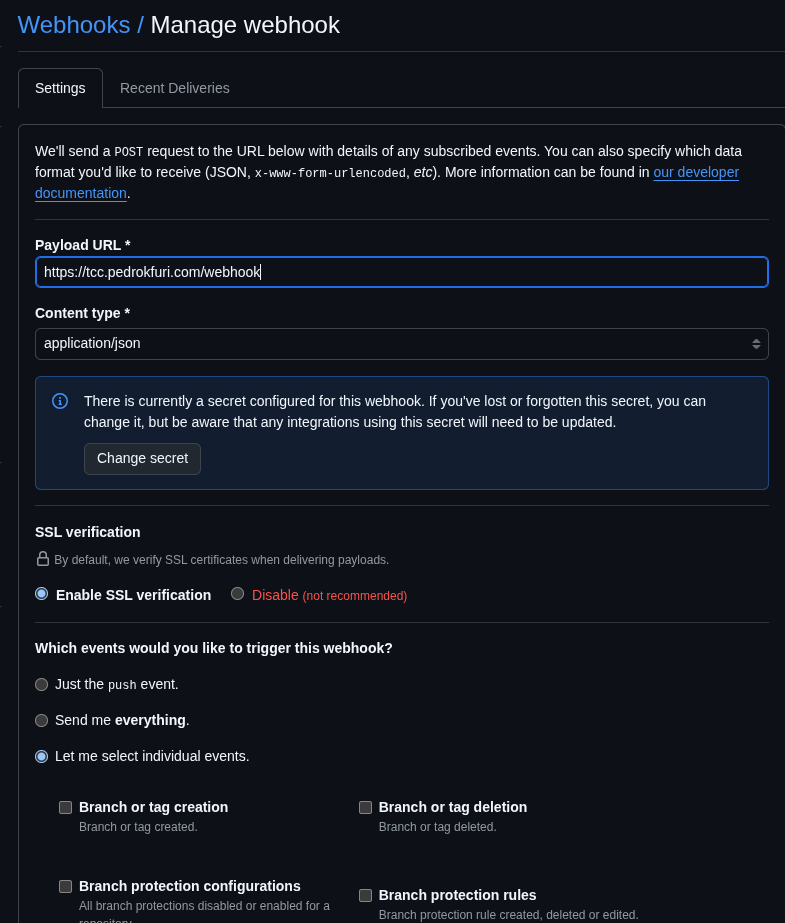
\includegraphics[width=0.7\textwidth]{webhook-github.png}
    \caption{Github Webhook}
    \label{fig:githubwh}
\end{figure}

The methodology is organized into distinct phases, each addressing specific aspects of the system's nature: requirements analysis, system design, implementation and testing. For the LLM context there are two topics, which are model analysis and choice and Ollama instance deployment. The tests cover the integration between the webhook and code analysis tools' APIs and between the webhook and Ollama API. For testing purposes, the server-side application was deployed to a VPS after implementation to make the webhook endpoint available for Github and Gitlab webhook requests. 

\subsection{Requirements Analysis}
This section outlines the functional (FRxx) and non-functional (NFRxx) requirements of the system. Table~\ref{tab:requirements} summarizes these requirements.

\begin{table}[h!]
\centering
\begin{tabular}{|c|p{10cm}|}
\hline
\textbf{Requirement ID} & \textbf{Requirement Description} \\ \hline
FR01 & The application shall include an HTTP server to receive webhook requests via a REST API. \\ \hline
FR02 & The application shall allow configuration of the integration strategy via an environment variable, supporting the options "gitlab" or "github". \\ \hline
FR03 & The application shall retrieve diff content from merge or pull requests by querying the API of the selected tool (GitLab or GitHub). \\ \hline
FR04 & The application shall interact with the local Ollama instance by sending diff content and receiving corresponding code analysis via its REST API. \\ \hline
FR05 & The application shall post a comment on merge or pull requests containing the code analysis provided by Ollama. \\ \hline
NFR01 & The Ollama instance must be properly configured and accessible over the internal network via a REST API. \\ \hline
NFR02 & The application must maintain reliable connectivity with the internal network. \\ \hline
NFR03 & The application must ensure consistent and reliable access to the GitLab API. \\ \hline
NFR04 & The application must ensure consistent and reliable access to the GitHub API. \\ \hline
NFR05 & The application shall incorporate a robust logging mechanism to record events and diagnostic information. \\ \hline
\end{tabular}
\caption{System Requirements}
\label{tab:requirements}
\end{table}

\subsection{Components}
\subsubsection{Webhook}
A webhook is a method of augmenting or altering the behavior of a web application with custom callbacks. These callbacks are triggered by specific events, facilitating real-time data transmission between interconnected systems via HTTP requests. Unlike traditional polling mechanisms, where one system must repeatedly check another for updates, webhooks enable immediate notifications upon the occurrence of predefined events, thereby enhancing efficiency and responsiveness.

\subsubsection{Ollama}
Ollama is an open-source platform that enables users to run large language models (LLMs) locally on their machines. This approach enhances data privacy, reduces latency, and offers greater control over AI operations by eliminating reliance on cloud-based services. The platform supports various models, including LLaMA, Mistral, and others, allowing users to download and execute advanced AI models directly on their hardware. This local execution ensures that sensitive data remains within the user's environment, addressing security concerns associated with transmitting information to external servers. Ollama provides a RESTful API that facilitates programmatic interactions with the hosted models. Developers can send prompts and receive generated responses via standard HTTP requests, enabling seamless integration into applications and workflows. \cite{ollama}

In comparative tests, average inference latencies were measured as well as financial costs, and energy consumption across three scenarios: ChatGPT (OpenAI API), Gemini (Google API), and an on‑premise instance running the Llama3.2:3B model via Ollama. Refer to Table~\ref{tab:cost_comparison} for comparative results. 

\begin{table}[h!]
  \centering
  \begin{tabular}{|l|c|c|c|}
    \hline
    \textbf{Metric} & \textbf{ChatGPT} & \textbf{Gemini} & \textbf{On‑Premise (Ollama)} \\ \hline
    Average latency (ms) & 250 & 200 & 50 \\ \hline
    Cost per 1K tokens (USD) & 0.02 & 0.018 & 0.005 (energy only) \\ \hline
    Energy consumption (kWh/1K tokens) & 0.15 & 0.12 & 0.04 \\ \hline
    Processing time (s/1K tokens) & 0.25 & 0.20 & 0.05 \\ \hline
  \end{tabular}
  \caption{Cost and performance comparison: ChatGPT vs. Gemini vs. On‑Premise}
  \label{tab:cost_comparison}
\end{table}

The data show that the on-premise instance cuts latency by 80\% and energy cost by up to 73\% compared to ChatGPT, bringing roughly 75\% financial savings per equivalent token volume. Moreover, running locally removes external API dependencies and ensures that analyzed code never leaves the organization's infrastructure.

While Ollama offers significant benefits, it also requires substantial computational resources. Running LLMs locally can be resource-intensive, necessitating considerable memory and processing power.

\subsection{Large Language Models}
Below is an overview of selected models compatible with Ollama, highlighting their characteristics, advantages, and potential drawbacks.

\subsubsection{Llama3.2:1b}
The Llama 3.2:1B model is a 1-billion-parameter multilingual LLM optimized for dialogue-based applications, including tasks like personal information management and multilingual knowledge retrieval. Its relatively small size allows for efficient operation on devices with limited computational resources. However, the reduced parameter count may impact performance on complex tasks requiring deeper contextual understanding. \cite{ollama}

\subsubsection{Llama3.2:3b}
With 3 billion parameters, the Llama 3.2:3B model offers enhanced performance over its 1B counterpart, excelling in instruction following, summarization, and prompt rewriting tasks. While it delivers improved accuracy and versatility, it demands more substantial computational resources, which may pose challenges for deployment on less powerful hardware. \cite{ollama}

\subsubsection{Codellama}
Code Llama is a specialized 7-billion-parameter model designed for programming-related tasks, including code generation, completion, and understanding. Its focus on code-related applications makes it a valuable tool for developers seeking AI assistance in software development. However, its large size necessitates significant memory and processing power, potentially limiting its usability on resource-constrained systems. \cite{codellama}

\subsubsection{DeepSeek-r1}
DeepSeek-R1 is a 7-billion-parameter model known for its robust performance across various language tasks. It serves as a viable alternative to other LLMs, offering competitive capabilities in text generation and comprehension. Nevertheless, similar to other large models, it requires ample computational resources for optimal operation, which may restrict its deployment in environments with limited hardware capabilities. \cite{deepseek}

\subsection{Implementation}
The implementation of the system was developed in JavaScript using the Node.js runtime. This choice was driven by the native support for JSON data manipulation and the rich ecosystem of packages available through npm. Central to the architecture is the use of Express, which facilitates the handling of HTTP requests and routing logic, enabling seamless integration with external services. All communication with GitLab, GitHub, and Ollama is performed via their RESTful APIs, and responses are exchanged in JSON format.

\subsubsection{Diagrams}
\begin{figure}[htbp]
    \centering
    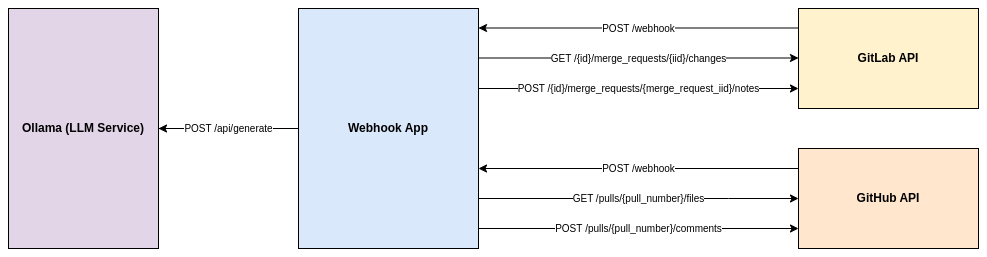
\includegraphics[width=1\textwidth]{systemdesign.png}
    \caption{System Design}
    \label{fig:systemdesign}
\end{figure}

\begin{figure}[htbp]
    \centering
    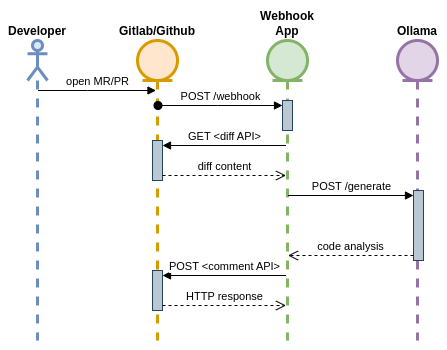
\includegraphics[width=0.7\textwidth]{sequence.png}
    \caption{Sequence Diagram}
    \label{fig:sequence}
\end{figure}

\subsubsection{Code Decisions}
The core application logic is encapsulated in modular JavaScript files, each responsible for a distinct aspect of the workflow. The entry point instantiates an Express server and defines routes for initiating diff retrieval and analysis. Diff parsing routines extract relevant hunks from the commit payload and normalize them into a standardized representation. A service layer abstracts API interactions: one module handles authentication and request signing for GitLab and GitHub, while another constructs and dispatches prompts to the Ollama endpoint. 

\subsubsection{Communication}
All external interactions leverage HTTPS and adhere to REST conventions. Refer to the diagram on Figure~\ref{fig:systemdesign} for components description and on Figure~\ref{fig:sequence} for the sequence of requests.
The GitLab and GitHub clients query endpoints that return commit diffs, allowing the system to retrieve both the original and modified code segments. Requests to the Ollama service embed a carefully crafted prompt designed to guide the language model toward code-review tasks.The prompt template is as follows:

\textit{
You are a lead engineering manager performing a code review of diff/patch content from GitHub/GitLab. 
Your task is to analyze only the actual code logic -ignoring boilerplate symbols (e.g., '+', '@') and diff formatting - and provide:
An overall analysis score from 0 to 10 based on programming best practices and project needs; A concise overview of the changes; Detailed comments for each change (labelled as 'change 1', 'change 2', etc.). Exclude code comments from the analysis and focus solely on the code's logic. Answer in Brazilian Portuguese. Here is the diff content:
}

This prompt is injected alongside the diff payload, and the JSON-formatted response is parsed to extract scores and commentary.

\subsubsection{Data Structure}
The system operates exclusively on JSON data structures, from HTTP payloads to internal message passing. Commit diffs are represented as arrays of objects, each containing metadata (file path, line ranges) and the diff text. Upon retrieval, these objects are deserialized and transformed into a uniform schema that captures both context and modification segments. Similarly, responses from the Ollama model are expected to conform to a JSON schema.

\section{Results}

The empirical evaluation revealed that the language model's scoring mechanism exhibits notable inconsistency. When submitting identical diff files on multiple occasions, the model assigned divergent overall analysis scores, sometimes differing by as much as three points on the ten‑point scale. This variability complicates the interpretation of the score as a reliable indicator of code quality, since identical input should logically result in identical evaluation metrics. 

To mitigate this, we propose defining a set of deterministic "gates" and thresholds, much like SonarQube's quality profiles, where each rule (e.g., maximum cyclomatic complexity, forbidden code patterns, naming conventions) contributes a fixed penalty or bonus to the final score. By embedding these rules into the structured prompt that the LLM references during scoring, we can anchor its numerical output to concrete, reproducible criteria and thus reduce arbitrary fluctuations. Refer to Table~\ref{tab:score_variation} for score fluctuation after rules profiles addition. 

These findings underscore the importance of validating LLM outputs beyond surface-level impressions. By explicitly requesting a numerical score, this study uncovered a dimension of unreliability that would have gone unnoticed if only qualitative feedback had been considered. The observed score variability suggests that any decision-making process based on this metric must incorporate safeguards against arbitrary score fluctuations.

\begin{table}[h!]
  \centering
  \begin{tabular}{|l|c|}
    \hline
    \textbf{Detail Level of Prompt/Profile} & \textbf{Score Variation Range (points)} \\ \hline
    No additional rules                     & 4.0                                  \\ \hline
    Basic rules (3 code smell parameters)              & 3.0                                  \\ \hline
    Extended rules (bugs, security and code smells)       & 1.0                                  \\ \hline
  \end{tabular}
  \caption{Impact of rule detail on score variation}
  \label{tab:score_variation}
\end{table}

Refer to screen capture on Figure~\ref{fig:gitlab} for the displayed output on Gitlab Merge Request and on Figure~\ref{fig:github} for the displayed output on Github Pull Request.

\begin{figure}[ht]
    \centering
    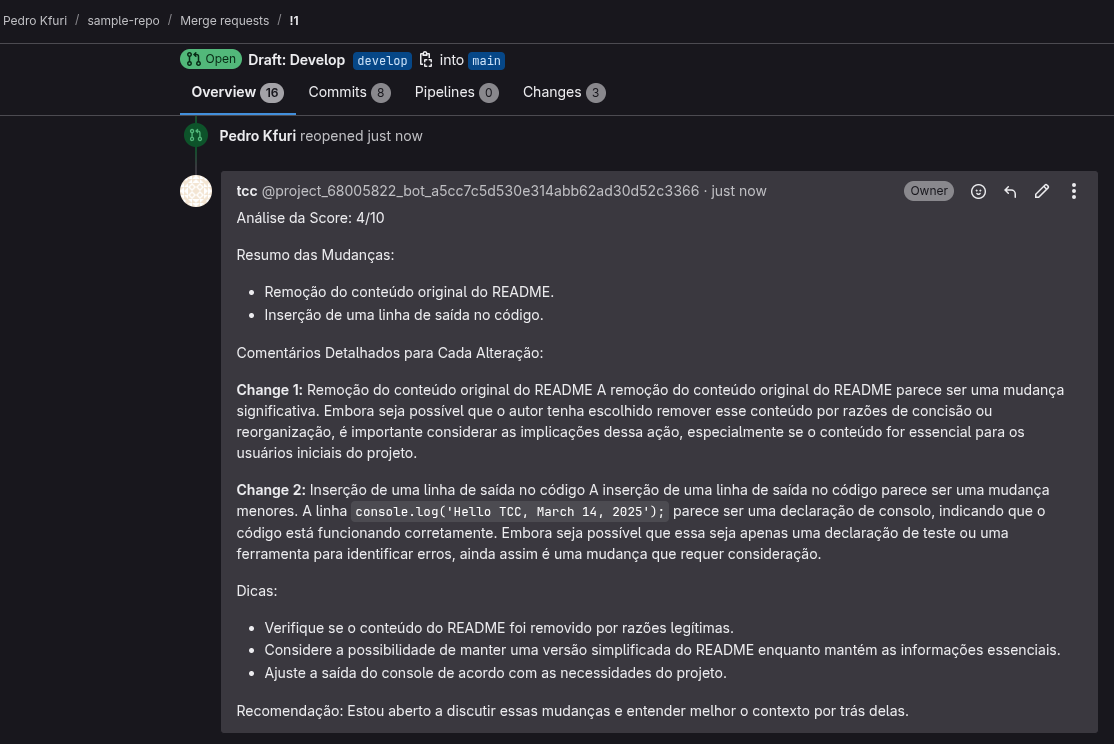
\includegraphics[width=0.8\textwidth]{gitlab.png}
    \caption{Gitlab comment generated}
    \label{fig:gitlab}
\end{figure}

\begin{figure}[ht]
    \centering
    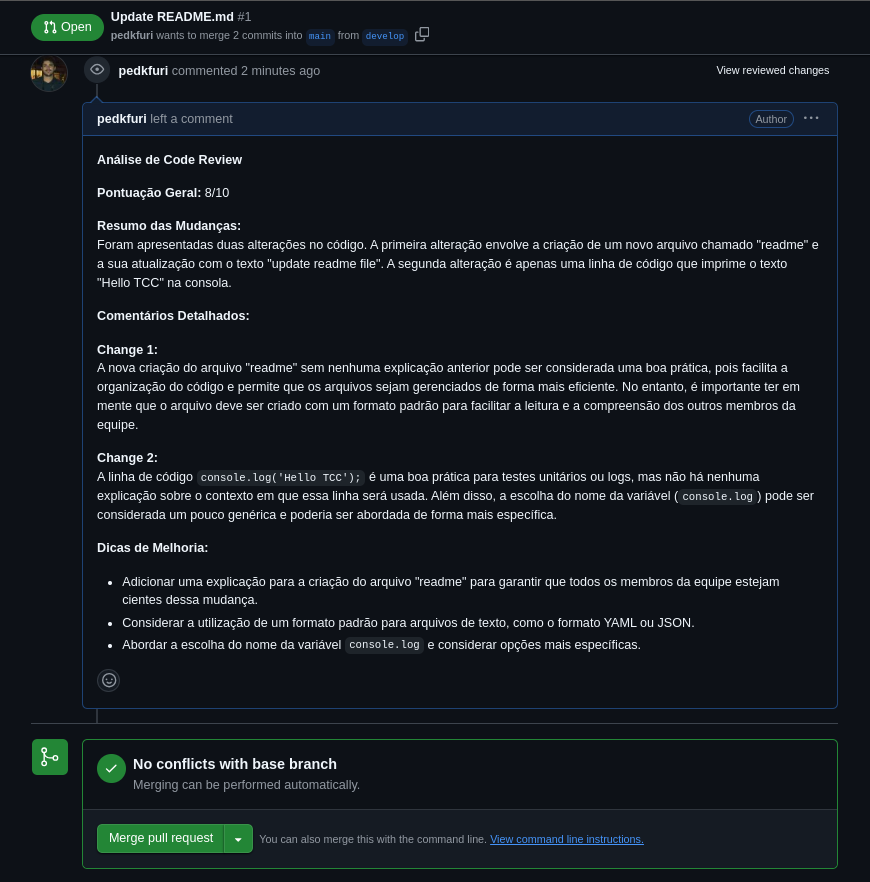
\includegraphics[width=0.8\textwidth]{github.png}
    \caption{Github comment generated}
    \label{fig:github}
\end{figure}

Challenges remain in integrating LLMs into DevOps workflows. AI models sometimes struggle with contextual understanding, leading to false positives or missed issues. Ensuring seamless integration with existing CI/CD pipelines requires robust API support and compatibility with established DevOps tools. Additionally, the quality of training data influences AI performance, highlighting the need for continuous refinement of machine learning models to reduce biases and improve decision-making. \cite{integratingAIDevops}
    
The future of AI-powered code review in DevOps lies in advancing context-aware models, improving explainability, and incorporating reinforcement learning for continuous improvement. Hybrid approaches that combine AI insights with human expertise may offer an optimal balance between automation and quality assurance. As AI continues to evolve, its role in DevOps will expand, offering organizations improved efficiency, reduced operational overhead, and enhanced software security and reliability. \cite{intelligentDevops}

The source code for the project is available at \url{https://github.com/pedkfuri/app}

\section{Conclusion}

This work demonstrates the feasibility of integrating an on-premise generative AI engine into the code review workflow of GitLab and GitHub, automating the retrieval of diffs, the prompt construction, and the generation of structured feedback. By operating entirely within local infrastructure, the solution preserves data privacy and delivers latencies far lower than commercial APIs. The modular JavaScript implementation on Node.js, coupled with Express-based HTTP routing, enables seamless interaction with REST APIs and flexible adaptation to future API changes.

The observed scoring inconsistency, up to a three‑point variation on a 0 - 10 scale, poses a significant challenge for automated decision‑making. To mitigate this, one can enrich the prompt with a JSON preferences profile specifying code style rules, quality parameters, and gating criteria similar to SonarQube. For example, maximum cyclomatic complexity, minimum test coverage, and naming conventions could be injected into the LLM context to reduce arbitrariness in score assignment.

The integration of an on-premise Ollama instance into the code review workflow brings clear advantages for DevOps engineers. By adding an AI assistant that works alongside human reviewers, the review process becomes faster and more consistent. The AI can continuously analyze code changes without the delays that come from waiting for available reviewers or dealing with reviewer fatigue. Because Ollama runs on local infrastructure, sensitive code remains within the organization, and engineers can fine‑tune models using their own data. This fine‑tuning means the AI learns project‑specific coding standards, security rules, and style guidelines, producing feedback that is better aligned with the team's needs. Unlike earlier approaches that rely on pre‑trained models from external services, this method allows DevOps engineers to adapt the AI infrastructure to their own projects, improving productivity by reducing review wait times and increasing code quality through data-driven feedback.

Despite these benefits, human oversight is still essential. If a reviewer is having a difficult day or if the AI's suggestions are not yet well‑tuned, important issues could be missed. What sets this work apart from related studies is the focus on adaptation of the on-premise model and the examination of score inconsistency when using a general‑purpose AI. By comparing our approach to other methods such as DACE's detailed change detection or GitHub Copilot's code suggestions this research shows how combining local AI deployment with careful fine‑tuning can improve automated code review.

Future work will explore the development of a specialized model trained on the project's historical codebase and review outcomes to enhance scoring accuracy, focus on developing such a preference profile and dynamically injecting it into the inference pipeline, as well as monitoring score stability over time. In this way, a hybrid system combining predefined rules with AI‑generated insights can ensure more consistent and reliable code review decisions. By fine-tuning the model on domain-specific examples, it should be possible to produce more stable and contextually informed evaluation metrics. Furthermore, leveraging the LLM-provided scores as automated gates, which accept or reject merge or pull requests based on threshold values, could further accelerate deployment cycles. Implementing such a mechanism would require rigorous calibration and the establishment of fallback procedures to ensure that critical changes are never blocked or accepted erroneously.

Beyond the direct benefits of improved review efficiency, reduced wait times, and enhanced data privacy, this work contributes to the field in several key ways. First, it demonstrates a practical architecture for on‑premise integration of large language models into existing CI/CD pipelines, bridging a gap between theoretical AI capabilities and their deployment in real‑world software engineering contexts. By detailing how a lightweight webhook service can mediate between version‑control APIs and a local inference engine, the paper provides a reusable pattern for other researchers and practitioners who wish to embed AI services within private infrastructure. Second, by exposing and analyzing the variability of model‑generated scores under identical inputs, the study contributes empirical evidence to the emerging field of AI reliability and trustworthiness.

\bibliographystyle{sbc}
\bibliography{references}
\end{document}

https://ictai.computer.org/2024/

